\documentclass{article}
\usepackage{graphicx}
\usepackage{float}
\begin{document}

\title{Depth and Volume}

\maketitle
\vspace{.5pc}

\section{Data}
We use historical data from the NYSE Trade and Quote database\footnote{We note that this data is known to have inaccuracies regarding quotes' timestamps, and such issues may carry over to trade timestamps. These issues stem from timestamps originating from a secondary source (i.e., not the exchanges' order matching engines) and being derived after an exchange aggregation method which introduces further latency\footnote{See Budish, Cramton and Shim (2015) and Ding, Hanna and Hendershott (2014)}.}, made available by Wharton Research Data Services. The dataset ``contains intraday transactions data (trades and quotes) for all securities listed on the New York Stock Exchange (NYSE), American Stock Exchange (AMEX), as well as Nasdaq National Market System (NMS) and SmallCap issues''\footnote{See https://wrds-web.wharton.upenn.edu/wrds/ds/taq/index.cfm.}.\\

Our data cover all trades for a sample of symbols\footnote{Our sample of symbols consists of AMD, BAC, C, GOOG, GRPN, JBLU, MSFT, and RAD. We would like to include BRKA and BRKB, but millisecond TAQ data does not exist for them. Strange.} over the period of Jan 1, 2014 - Dec 31, 2014. No time filtering is used, and we are left with a total of 249 trading days.\\

\subsection{Trades Data}
The trading data is organized as a sequential collection of trades, where a trade is defined as a transaction with a unique trade sequence number. A trade must be between no more than two parties, in one symbol, at one price, on one exchange, at one time.\\
Since we filter out some special cases (trade corrections, duplicates, etc.), we will not go into that here.\footnote{www.nyxdata.com/doc/224904}\\

\subsubsection{Trades Against One Counterparty}
Alice buys 50 shares of GOOG for \$700 on NASDAQ at 11:00 against a corresponding quote of at least 50 shares. The trades data would show the following:
\begin{center}
  \begin{tabular}{| c | c | c | c | c |}
    \hline
    Time & Symbol & Volume & Price & Exchange \\ \hline
    11:00:00 & GOOG & 50 & \$700.00 & NASDAQ \\
    \hline
  \end{tabular}
\end{center}
\subsubsection{Trades Against Multiple Counterparties}
Alice sells 50 shares of GOOG for \$700 on NASDAQ at 11:00, but the first-in-line quote is only big enough for 10 shares. The next two quotes, however, are of size 6 an 80, respectively, and so Alica can be accommodated by these three quotes. The trades data would show the following:
\begin{center}
  \begin{tabular}{| c | c | c | c | c |}
    \hline
    Time & Symbol & Volume & Price & Exchange \\ \hline
    11:00:00 & GOOG & 15 & \$700.00 & NASDAQ \\ \hline
    11:00:00 & GOOG & 6 & \$700.00 & NASDAQ \\ \hline
    11:00:00 & GOOG & 29 & \$700.00 & NASDAQ \\
    \hline
  \end{tabular}
\end{center}
\subsubsection{Trades On Multiple Exchanges}
Alice sends a buy order 20 shares of GOOG for \$700 on NASDAQ and a buy order 30 shares of GOOG for \$700 on NYSE. Furthermore, the first-in-line quote on NYSE is only big enough for 1 share, but the next quote in the NYSE queue is for 100 shares. The trades data would show the following:
\begin{center}
  \begin{tabular}{| c | c | c | c | c |}
    \hline
    Time & Symbol & Volume & Price & Exchange \\ \hline
    11:00:00 & GOOG & 20 & \$700.00 & NASDAQ \\ \hline
    11:00:00 & GOOG & 1 & \$700.00 & NYSE \\ \hline
    11:00:00 & GOOG & 29 & \$700.00 & NYSE \\
    \hline
  \end{tabular}
\end{center}
\subsubsection{Trades At Multiple Prices}
Alice sends a market buy order for 50 shares of GOOG on BATS BYX. The first-in-line quote is to sell 3 shares at \$700, and the next quote in the queue is for 16 shares at \$700.01. The next quote is for 19 shares at \$700.01, and the following quote is for 60 shares at \$700.03. The trades data would show the following:
\begin{center}
  \begin{tabular}{| c | c | c | c | c |}
    \hline
    Time & Symbol & Volume & Price & Exchange \\ \hline
    11:00:00 & GOOG & 3 & \$700.00 & BATS BYX \\ \hline
    11:00:00 & GOOG & 16 & \$700.01 & BATS BYX \\ \hline
    11:00:00 & GOOG & 19 & \$700.01 & BATS BYX \\ \hline
    11:00:00 & GOOG & 12 & \$700.03 & BATS BYX \\
    \hline
  \end{tabular}
\end{center}
\subsubsection{Order Gets Routed}
Alice sends a market sell order for 50 shares of GOOG on BATS BYX. The first-in-line quote is to buy 5 shares at \$700, and the next quote in the queue is for 60 shares at \$699.98. However, NASDAQ is the national best bid with a size of 1 share at \$699.99. By Reg NMS, Alice's sell order gets routed to NASDAQ and she sells 1 share for \$699.99. Now, the national best bid is the 60 shares at \$699.98 on BATS BYX. Alice's order transacts her remaining 44 shares against the 60 share bid on BATS BYX. The trades data would show the following:
\begin{center}
  \begin{tabular}{| c | c | c | c | c |}
    \hline
    Time & Symbol & Volume & Price & Exchange \\ \hline
    11:00:00 & GOOG & 5 & \$700.00 & BATS BYX \\ \hline
    11:00:00 & GOOG & 1 & \$699.99 & NASDAQ \\ \hline
    11:00:00 & GOOG & 44 & \$699.98 & BATS BYX \\
    \hline
  \end{tabular}
\end{center}
\subsubsection{Trades At Different Times}
Alice buys 40 shares of GOOG for \$700 on BATS BYX at 11:00:00 against two orders of size 13 and 90, respectively. Bob then sells 10 shares of GOOG for \$699.97 on NASDAQ at 11:00:04. The trades data would show the following:
\begin{center}
  \begin{tabular}{| c | c | c | c | c |}
    \hline
    Time & Symbol & Volume & Price & Exchange \\ \hline
    11:00:00 & GOOG & 13 & \$700.00 & BATS BYX \\ \hline
    11:00:00 & GOOG & 27 & \$700.00 & BATS BYX \\ \hline
    11:00:04 & GOOG & 10 & \$699.99 & NASDAQ \\ 
    \hline
  \end{tabular}
\end{center}

\subsection{Quotes Data}
The quotes data is organized as a sequential collection of quote updates, which only occur when the best bid/offer (BBO) has changed. These changes could be the result of a trade, a quote addition, a quote retraction, or a quote modification.\\
The following scenarios are all for one symbol on one exchange, as their quotes data are independent of one another.\\

\subsubsection{Nothing Happens}
The market opens at 09:30 with a \$9.99 bid for 30 shares and a \$10.03 bid for 15 shares. This remains the BBO for the remainder of the day:
\begin{center}
  \begin{tabular}{| c | c | c | c | c |}
    \hline
    Time & Bid Size & Bid & Offer & Offer Size \\ \hline
    09:30:00 & 30 & \$9.99 & \$10.03 & 15 \\
    \hline
  \end{tabular}
\end{center}
\subsubsection{Improved Quotes}
The market opens at 09:30 with a \$9.99 bid for 30 shares and a \$10.03 bid for 15 shares. At 09:44:00, a new \$10.00 bid for 2 shares enters the market. At 10:20:00, a new \$10.02 offer for 30 shares enters the market. This remains the BBO for the remainder of the day:
\begin{center}
  \begin{tabular}{| c | c | c | c | c |}
    \hline
    Time & Bid Size & Bid & Offer & Offer Size \\ \hline
    09:30:00 & 30 & \$9.99 & \$10.03 & 15 \\ \hline
    09:44:00 & 2 & \$10.00 & \$10.03 & 15 \\ \hline
    10:20:00 & 2 & \$10.00 & \$10.02 & 30 \\
    \hline
  \end{tabular}
\end{center}
\subsubsection{Joined Quotes}
The market opens at 09:30 with a \$9.99 bid for 30 shares and a \$10.03 bid for 15 shares. At 09:48:00, a new \$9.99 bid for 20 shares enters the market, joining the existing bid for 30 shares. This remains the BBO for the remainder of the day:
\begin{center}
  \begin{tabular}{| c | c | c | c | c |}
    \hline
    Time & Bid Size & Bid & Offer & Offer Size \\ \hline
    09:30:00 & 30 & \$9.99 & \$10.03 & 15 \\ \hline
    09:48:00 & 50 & \$9.99 & \$10.03 & 15 \\ 
    \hline
  \end{tabular}
\end{center}
\subsubsection{Retracted (or Traded) Quotes}
The market opens at 09:30 with two \$9.99 bids for 10 and 20 shares, respectively, and a \$10.03 bid for 15 shares. At 09:33:00, the \$9.99 bid for 10 shares is retracted (or traded). At 09:34:00, the \$9.99 bid for 20 shares is retracted (or traded), and now the previously existing \$9.98 bid for 100 shares is the new best bid. This remains the BBO for the remainder of the day:
\begin{center}
  \begin{tabular}{| c | c | c | c | c |}
    \hline
    Time & Bid Size & Bid & Offer & Offer Size \\ \hline
    09:30:00 & 30 & \$9.99 & \$10.03 & 15 \\ \hline
    09:33:00 & 20 & \$9.99 & \$10.03 & 15 \\ \hline
    09:34:00 & 100 & \$9.98 & \$10.03 & 15 \\
    \hline
  \end{tabular}
\end{center}


\section{Transforming Data}
Each data point concerned a specific symbol $i$'s activity on a specific exchange $j$ for a specific date $t$.

\subsection{Volume}
Volume $Q_{ijt}$ is computed as the sum of the volumes $q$ of trades occurring between 10:00 and 15:30 in symbol $i$ on exchange $j$ on date $t$:\\
$$Q_{ijt} = \sum_{q \in ijt} q$$

\subsection{Depth}
We begin by computing the depth of each quote update, indexed by $u$. This is done by taking the size of the best bid $q_{bu}$ and the size of the best ask $q_{au}$ and taking their average $\overline{q_u}$:\\
$$\overline{q_u} = \frac{q_{bu} + q_{au}}{2}.$$\\
For each quote update $u$, we compute its duration $\Delta T_u$--that is, how long this quote update $u$ represents the actual state of the book. We do this by subtracting the timestamp $T_u$ of quote update $u$ from the timestamp $T_{u+1}$ of the next quote update $u+1$:\\
$$\Delta T_u = T_{u+1} - T_u.$$\\
To summarize the depth $\overline{d}_{ijt}$ between 10:00 and 15:30 in symbol $i$ on exchange $j$ on date $t$, we take the sum of $\overline{q_u}$ weighted by their corresponding $\Delta T_u$.\\
$$\overline{d}_{ijt} = \sum_{u \in ijt} q_u \cdot\Delta T_u$$

John mentioned how NASDAQ quotes effectively treat its different DMMs as different exchanges; make sure to do special logic for NASDAQ.

\section{Results}
Due to wide heterogeneity in volumes between symbols, we take the logarithm of both depth and volume.\\

We filter out data points with negative values, as this implies empty bids or asks. (Penalizing quotes past the NBBO should solve this problem.)\\

\begin{figure}[H]
\centering
\includegraphics[width=120mm]{{./../output/trends/TimeChartDollarShot}.png}
\caption{The values of daily depth and volume are plotted against each other across symbols. The colors correspond to different exchanges.}
\end{figure}

Graphs are located in Dropbox\footnote{https://www.dropbox.com/sh/kxtlz8mb4lzfvgl/AAACcauEobiX21IBCM\_\_6IUja?dl=0}.\\

For each date $t$, we fit the regression model:\\
$$\log{\overline{d}_{ijt}} = \alpha_t + \beta_{t} \cdot \log{Q_{ijt}} + \epsilon_{ijt}.$$\\

\subsection{$\beta_t$ Over All Exchanges and Symbols}
\begin{figure}[H]
\centering
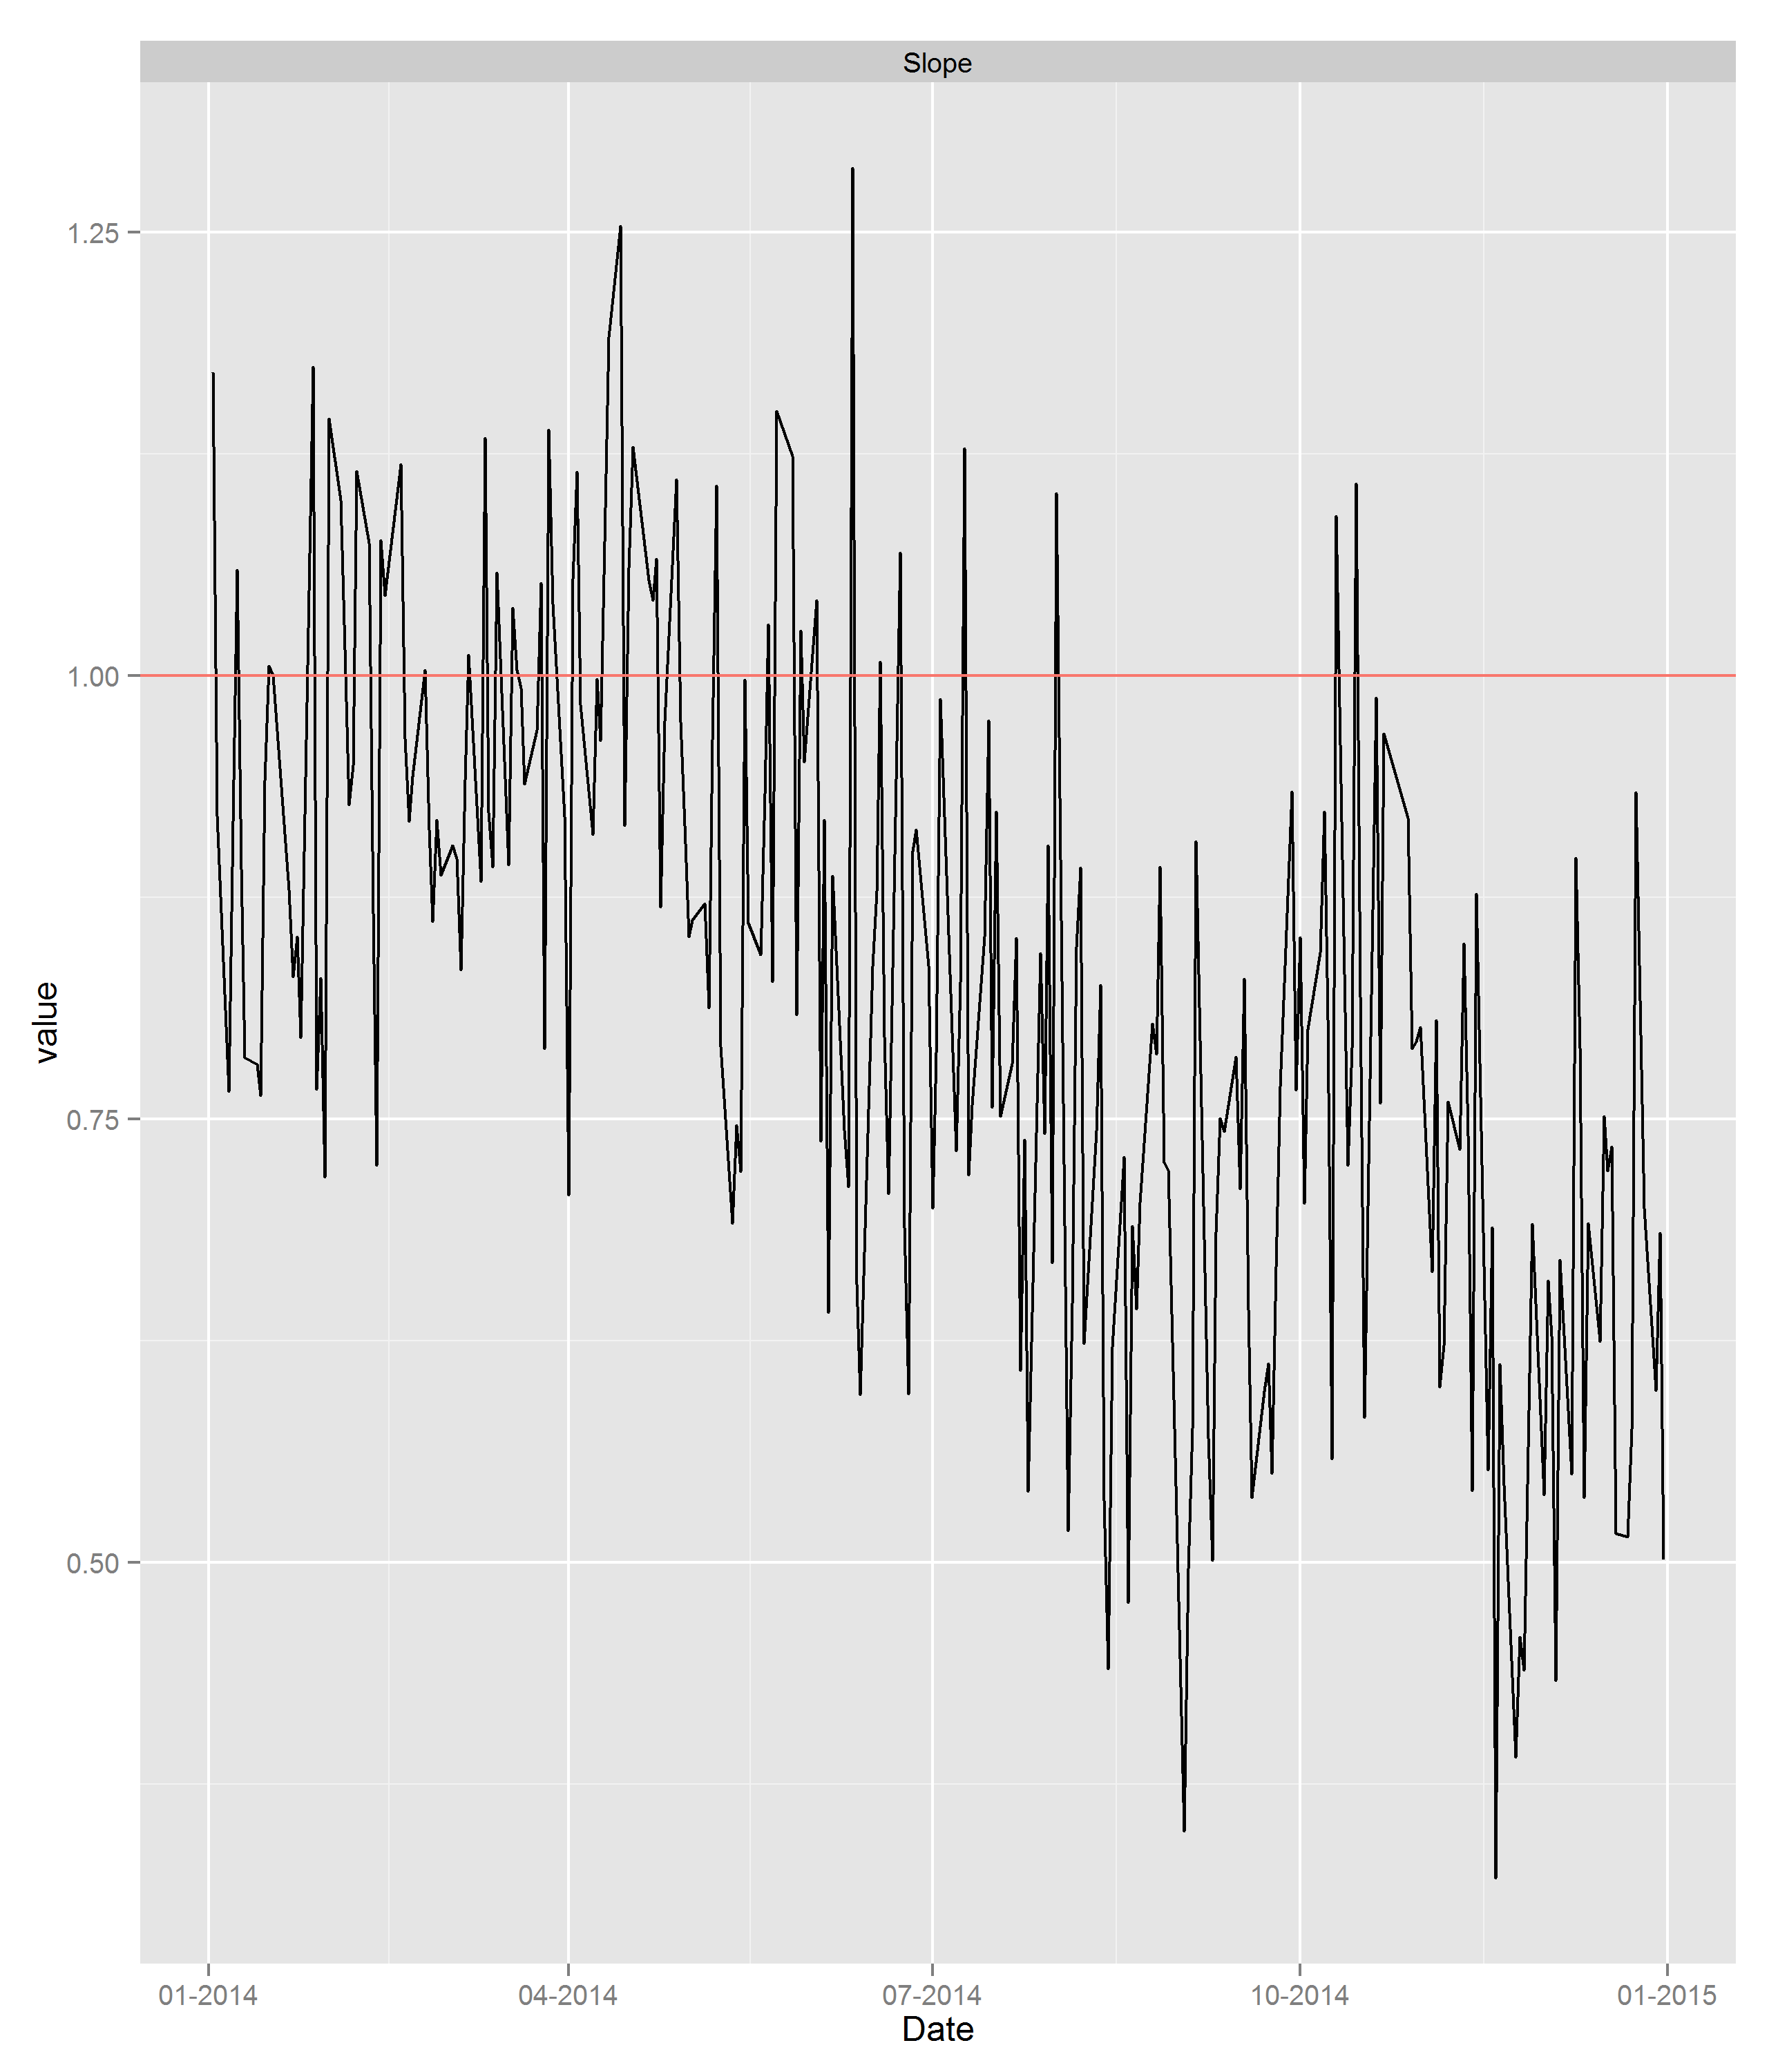
\includegraphics[width=120mm]{{./../output/trends/AllCoeffsTS}.png}
\caption{The values of $\beta_t$ over time without regard to exchange or symbol.}
\end{figure}
\begin{figure}[H]
\centering
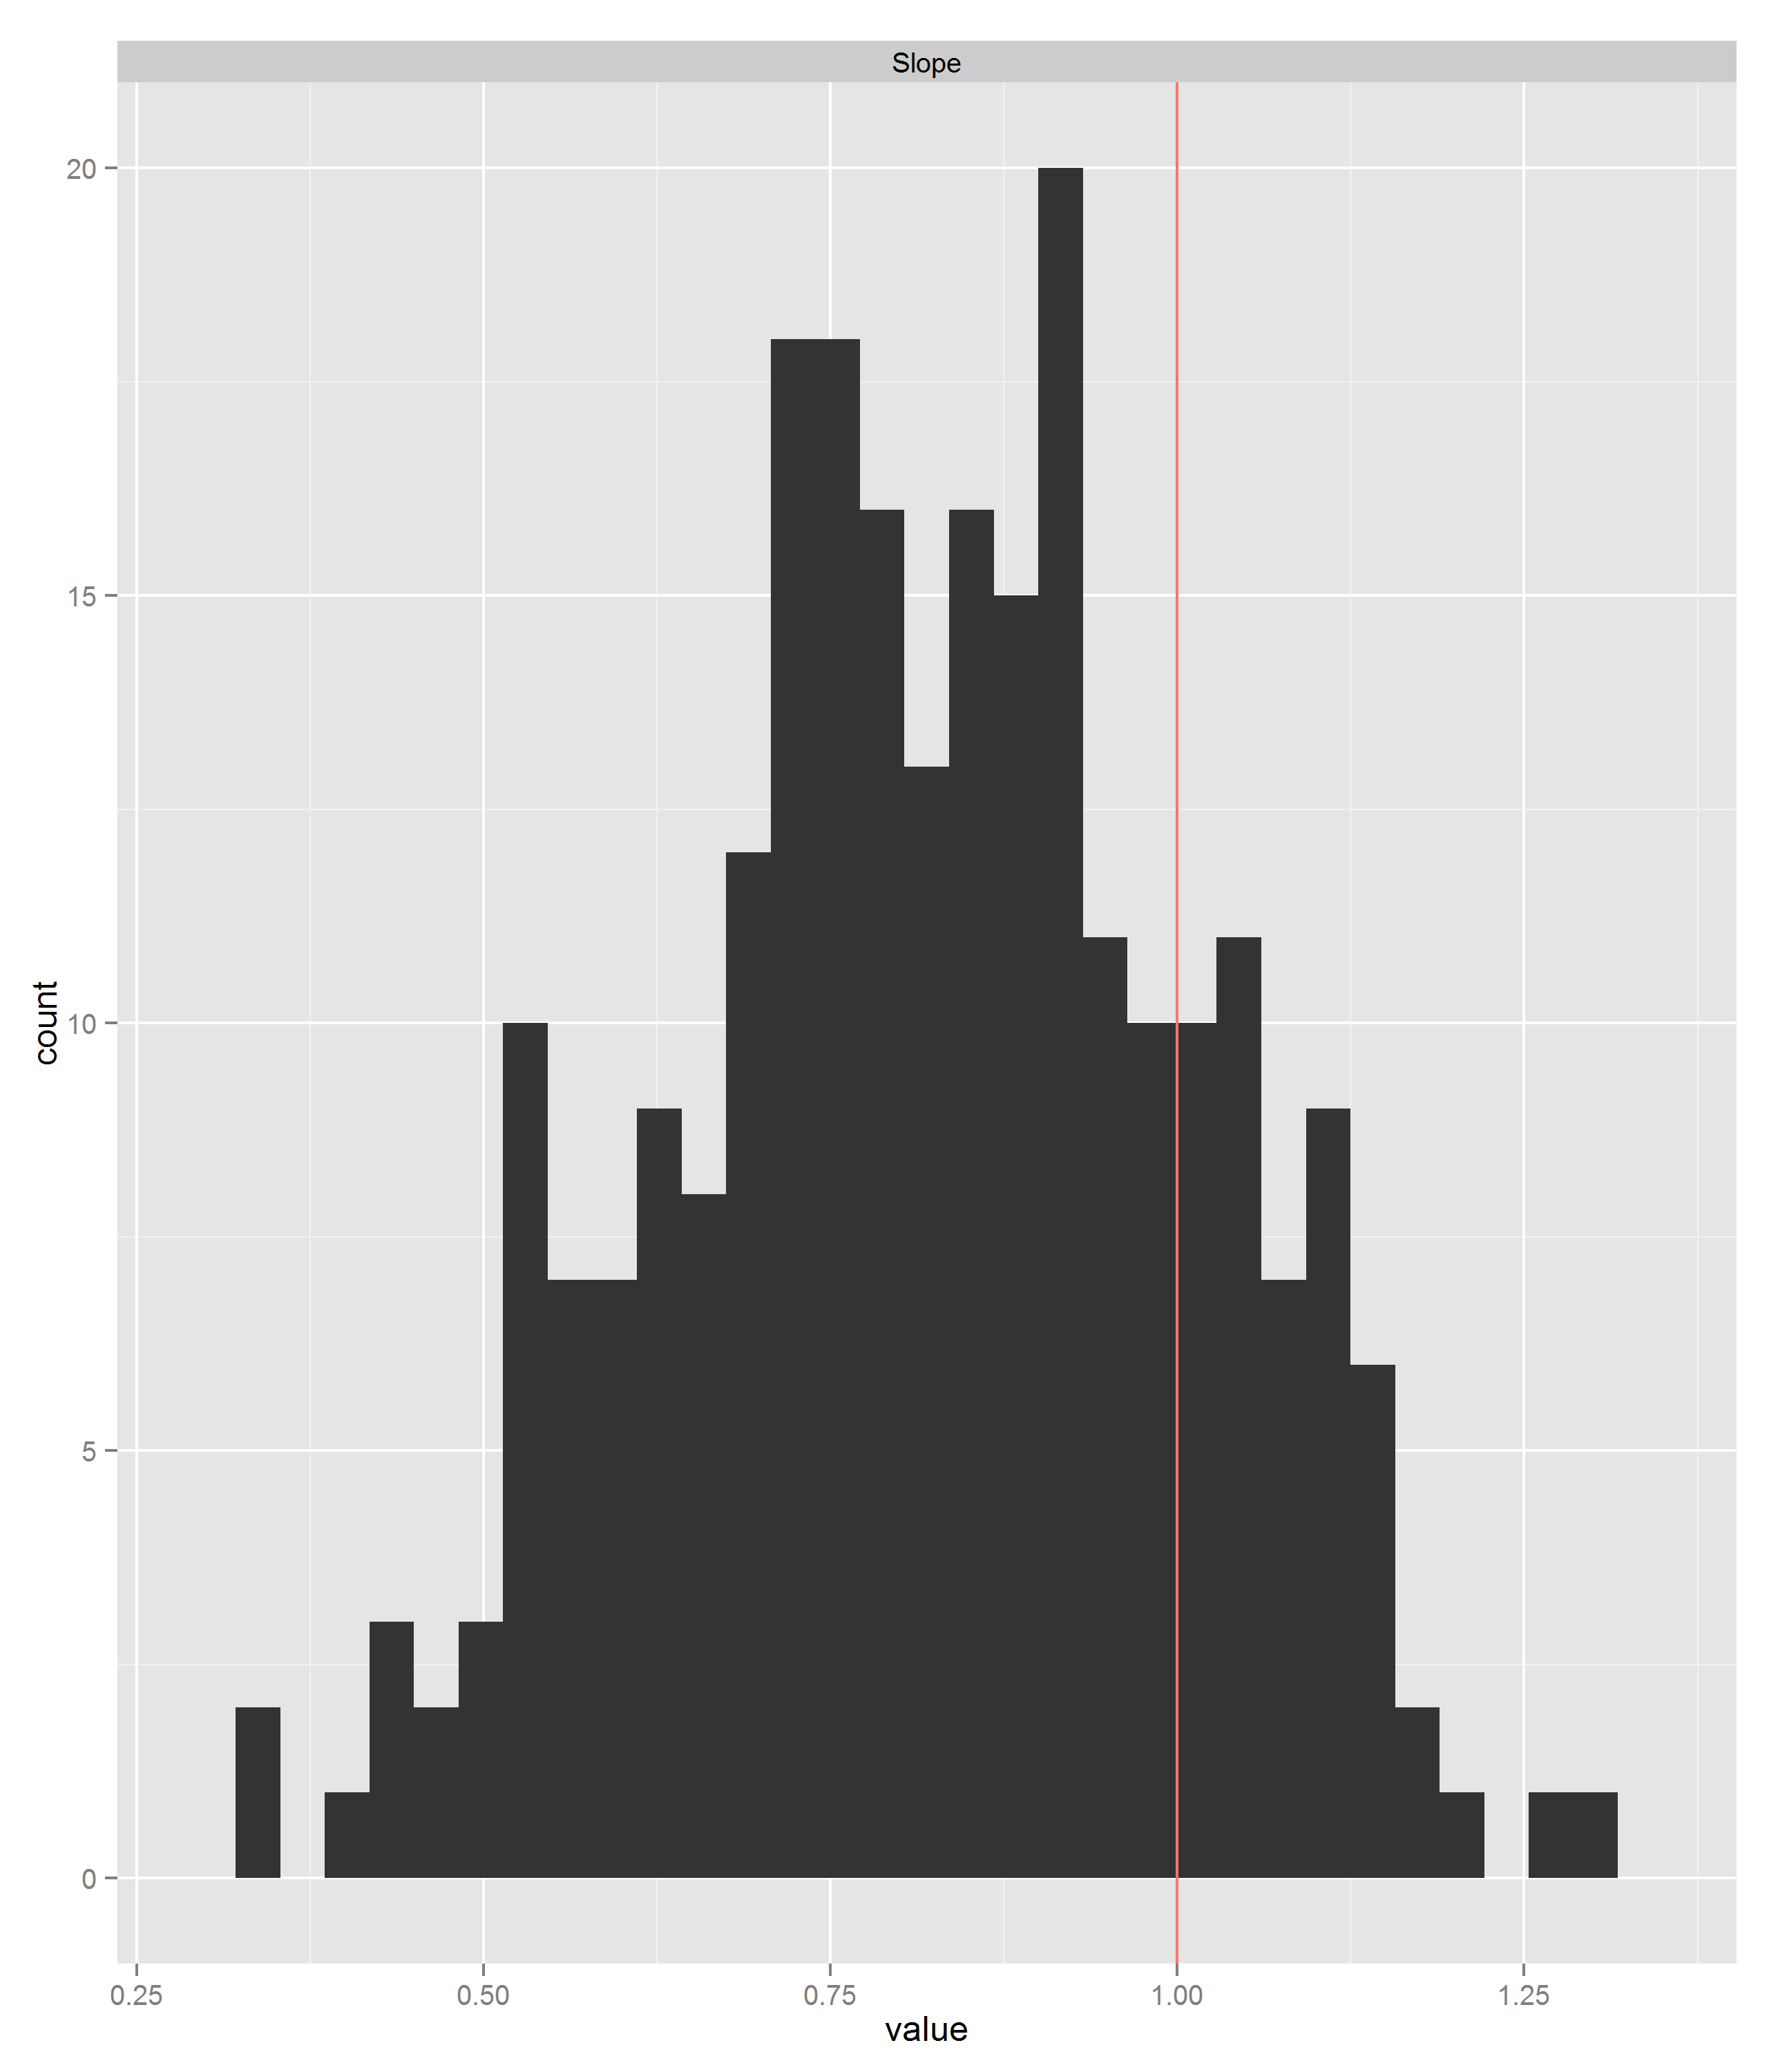
\includegraphics[width=120mm]{{./../output/trends/AllCoeffsHist}.png}
\caption{Histogram of $\beta_t$ without regard to exchange or symbol.}
\end{figure}

\subsection{$\beta_t$ Grouped by Exchange}
\begin{figure}[H]
\centering
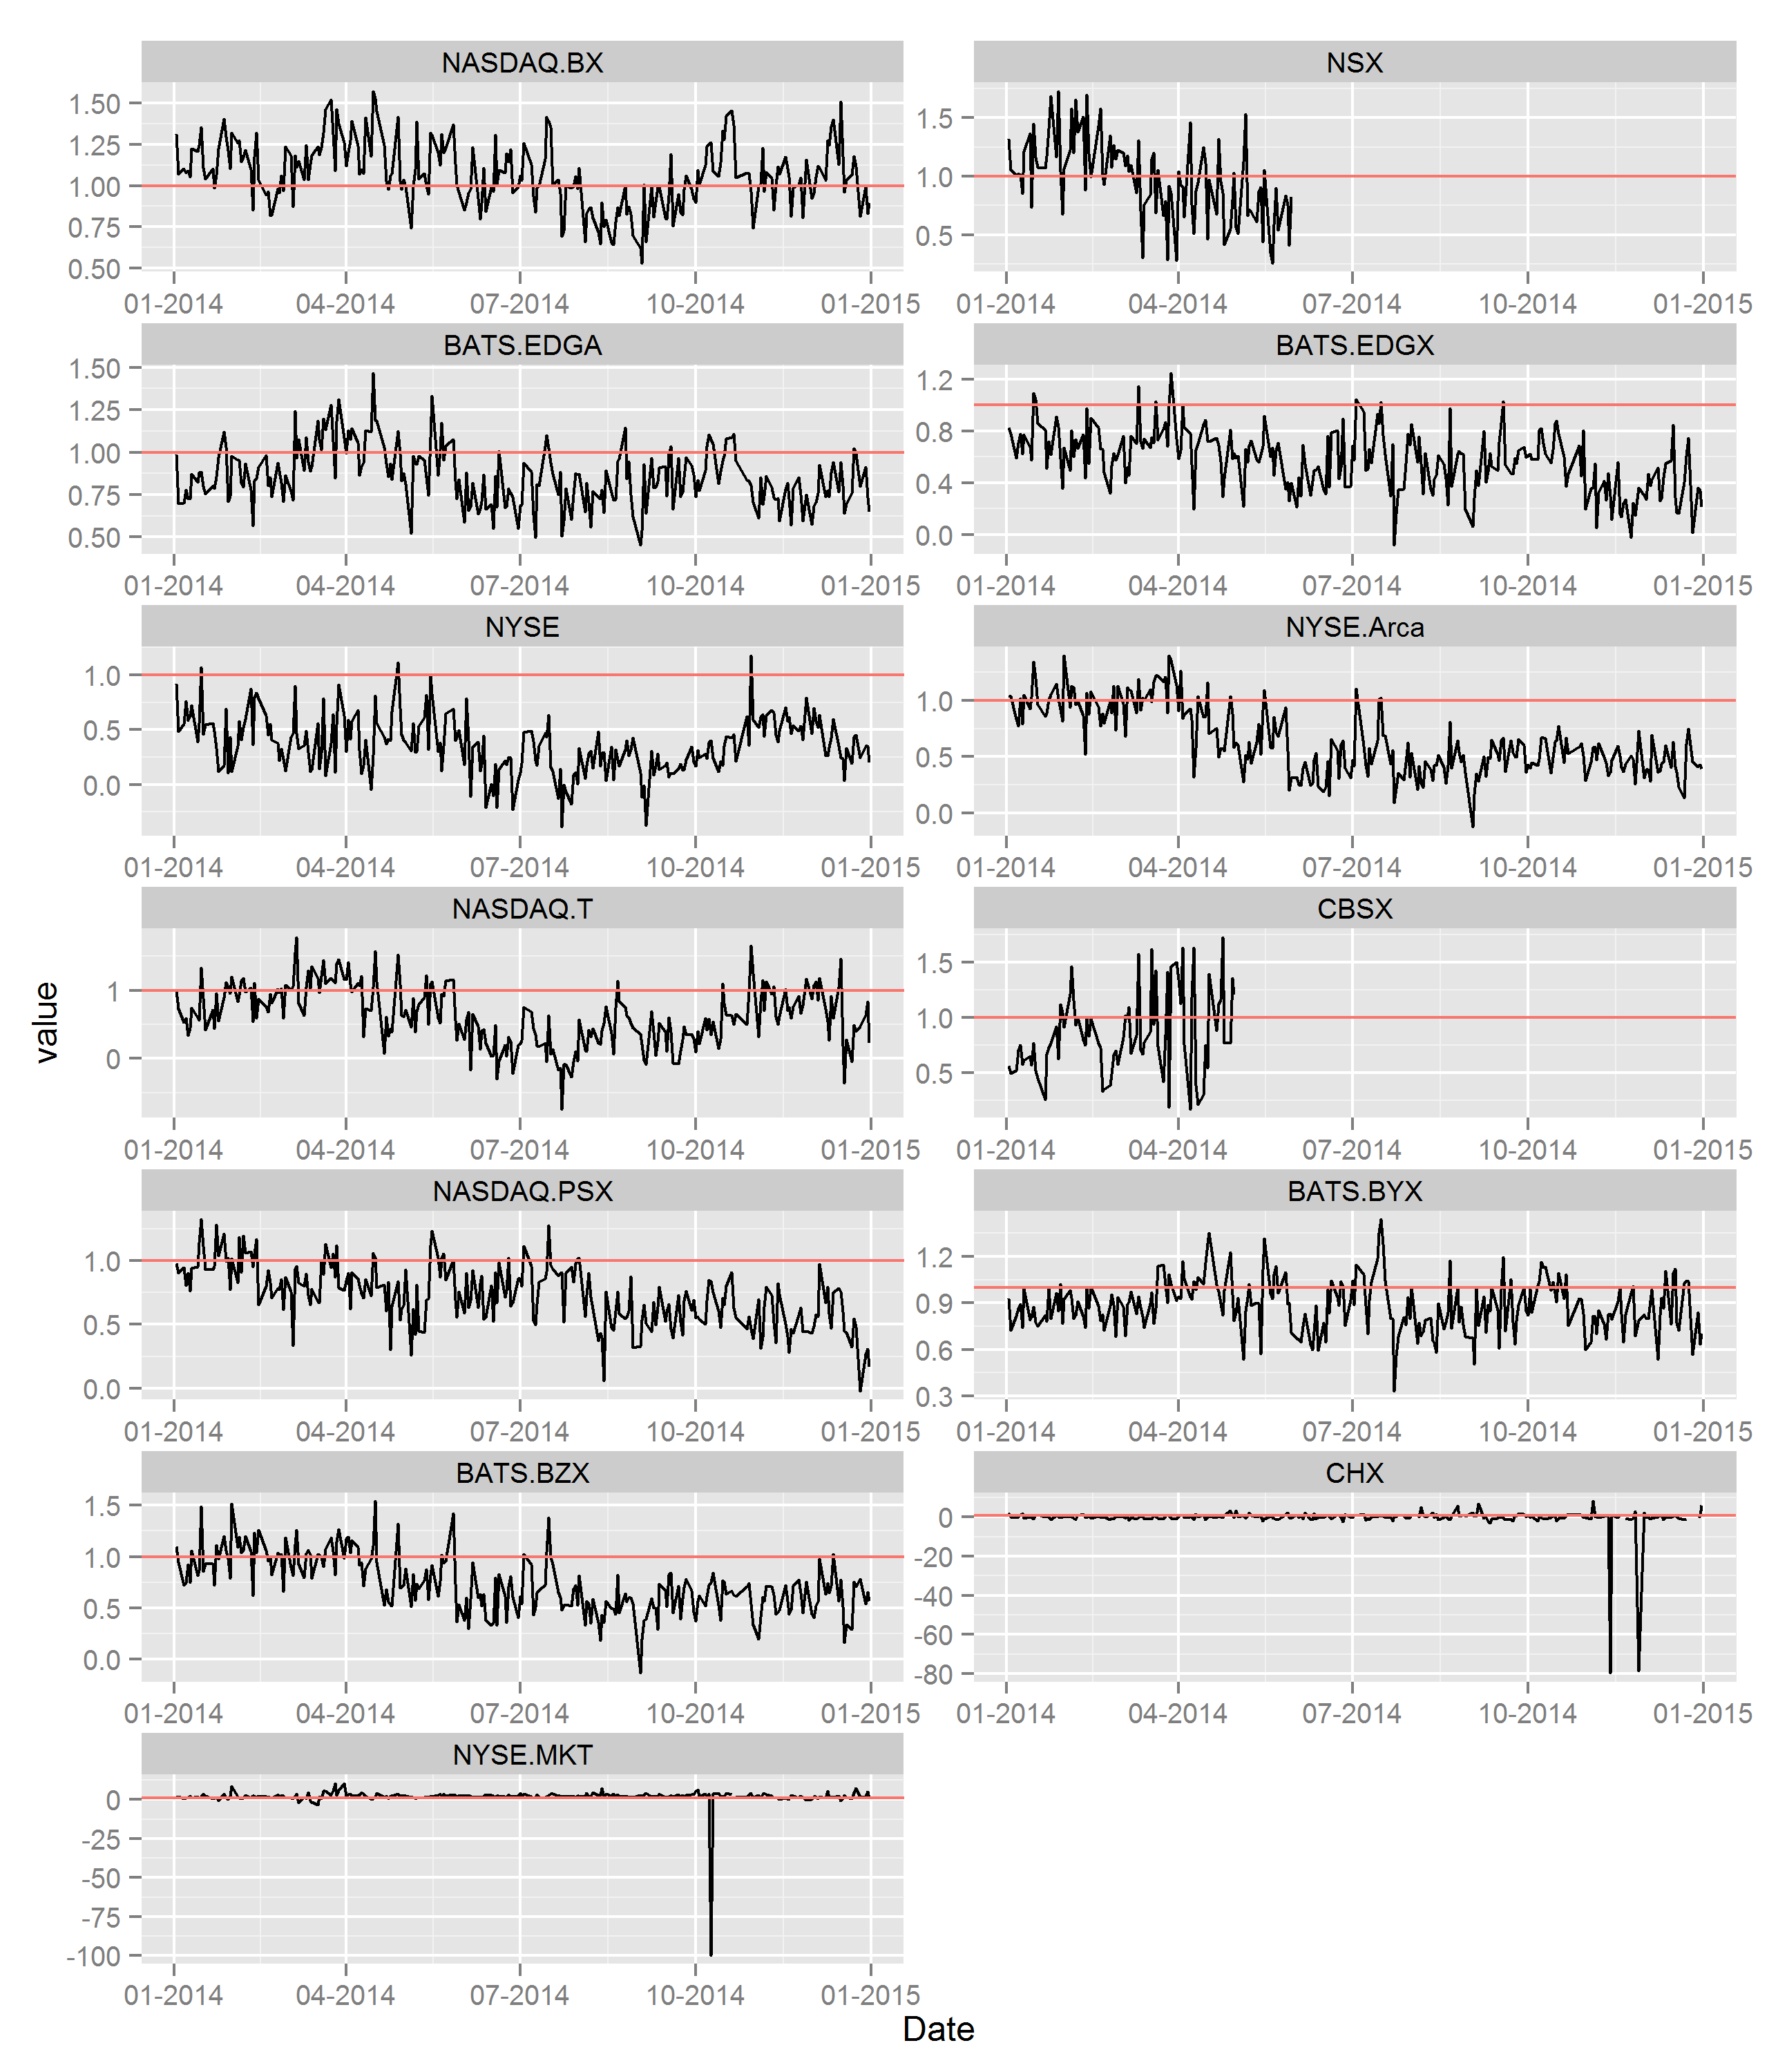
\includegraphics[width=120mm]{{./../output/trends/ExchangeCoeffsTS}.png}
\caption{The values of $\beta_t$ over time per exchange.}
\end{figure}
\begin{figure}[H]
\centering
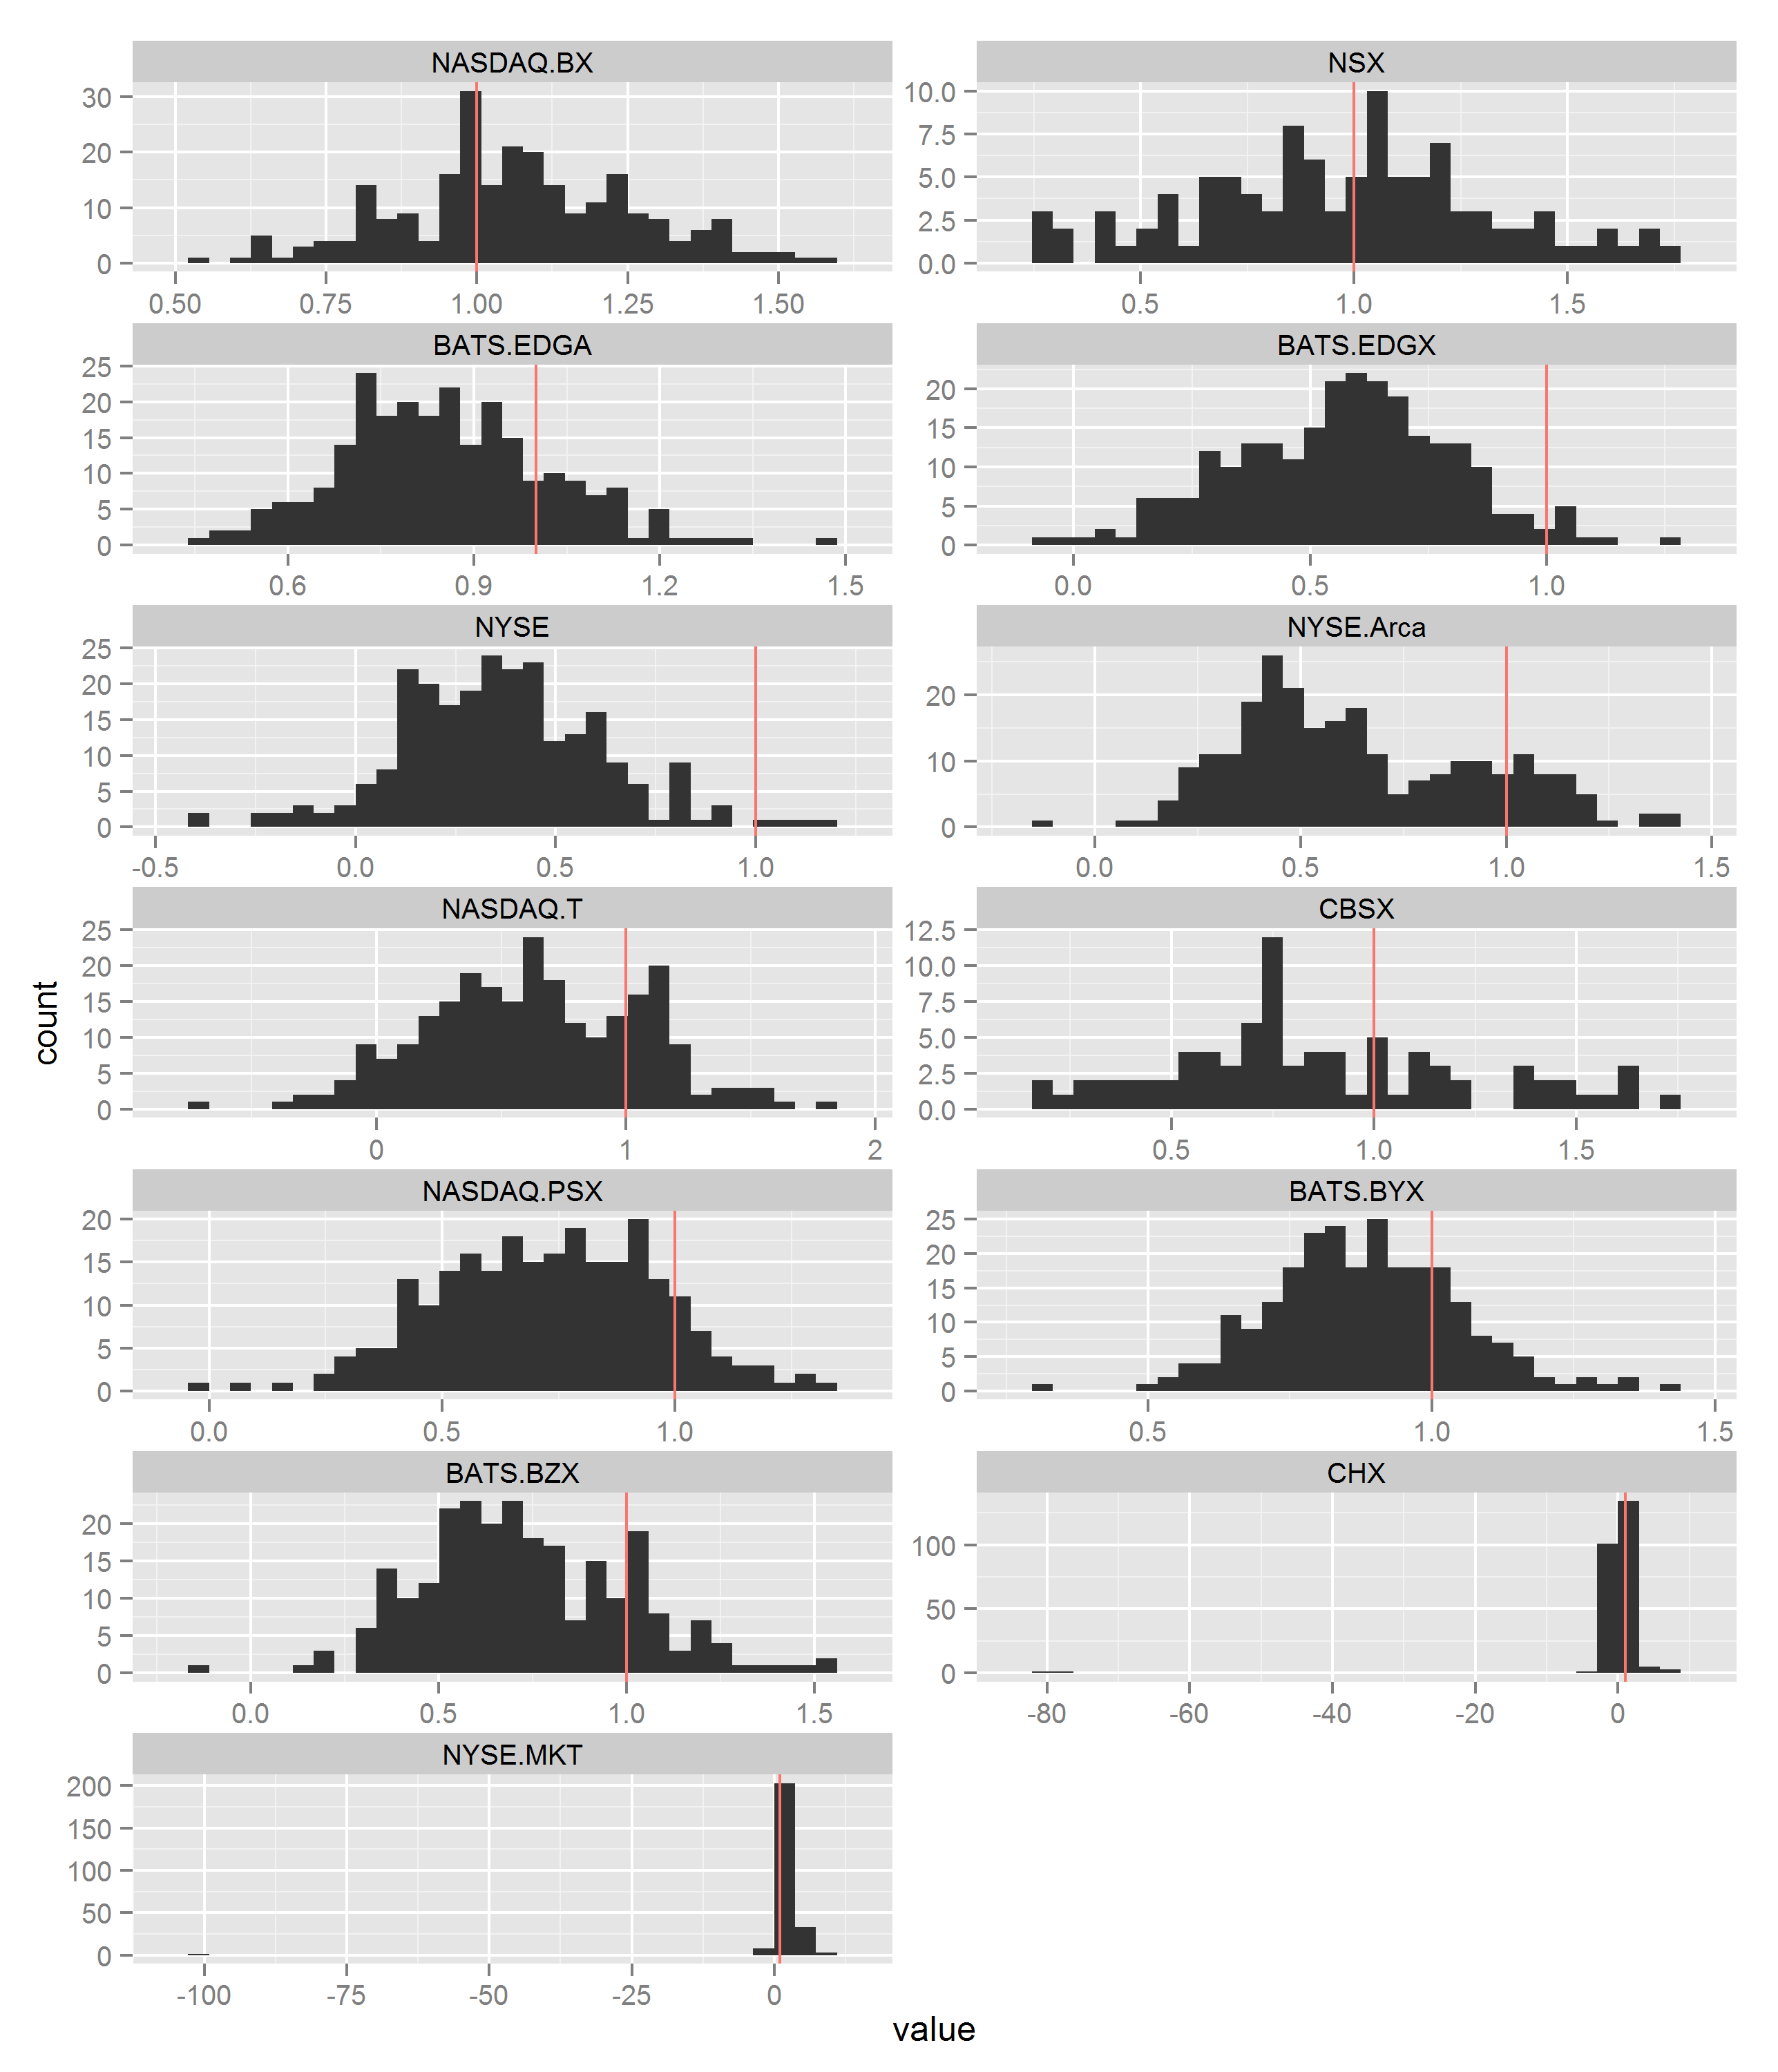
\includegraphics[width=120mm]{{./../output/trends/ExchangeCoeffsHist}.png}
\caption{Histogram of $\beta_t$ per exchange.}
\end{figure}
\subsection{$\beta_t$ Grouped by Symbol}

\begin{figure}[H]
\centering
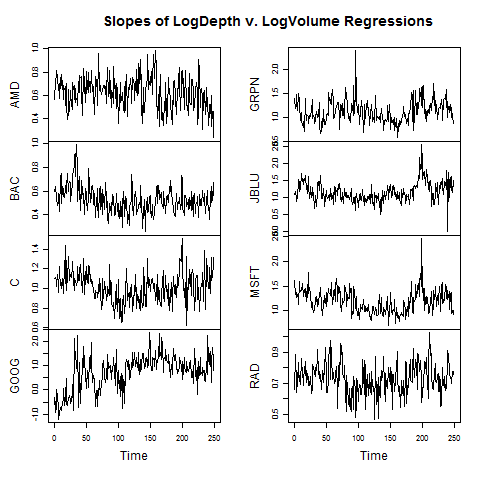
\includegraphics[width=120mm]{{./../output/trends/SymbolCoeffsTS}.png}
\caption{The values of $\beta_t$ over time per symbol.}
\end{figure}
\begin{figure}[H]
\centering

\includegraphics[width=120mm]{{./../output/trends/SymbolCoeffsHist}.png}
\caption{Histogram of $\beta_t$ per symbol.}
\end{figure}

\end{document}